\documentclass[german,10pt]{book}      \input{preambel}         \begin{document}  \setcounter{chapter}{0}

%\begin{document}  \setcounter
%\newcommand{\solution}[1]{}
\newcommand{\bra}[1]{\left.\langle #1\right |}
\newcommand{\ket}[1]{\left | #1\rangle\right.}
\newcommand{\braket}[2]{\langle #1 \left | #2\right.\rangle}
\newcommand{\mycomment}[1]{}

\chapter{Das Photon}
% Kap x
\label{chap_Photon}

\begin{picture}(0,0)(0,0)
\put(400,150){\makebox(0,0){
\includegraphics[scale=0.5]{./Bilder/bmftr.png}}}
\put(337,185){\makebox(0,0){\footnotesize Kurztext erstellt im Rahmen von \glqq Quanten auf Reisen\grqq}}
\end{picture}

\info{Anja Kuhnhold}{23.11.2025}\footnote{Bei der Überarbeitung und Gliederung dieses Textes, sowie der Erstellung von Abbildungen wurde ChatGPT zu Rate gezogen (Zugang: HAWKI, https://hawki.uni-freiburg.de/interface, ChatGPT-4.1 (Provider: Firma OpenAI), bzw.\ Open WebUI, https://openwebui.uni-freiburg.de/ OpenAI: ChatGPT-5/5.2/5.4).}

\section{Beschreibung von Licht}
In der Schule begegnet man Licht oft zun\"achst im Strahlenmodell. Im Laufe der Physikgeschichte wurden verschiedene Modelle entwickelt, um unterschiedliche Aspekte des Lichts zu beschreiben. F\"ur die vorliegende Darstellung sind vor allem zwei Modelle wichtig.
Im klassischen Bild wird Licht als elektromagnetische Welle beschrieben, die sich im Vakuum mit Lichtgeschwindigkeit ausbreitet.
Ihr Verhalten wird durch die Maxwell-Gleichungen beschrieben.
Lichtwellen k\"onnen sich \"uberlagern und interferieren; au{\ss}erdem k\"onnen sie polarisiert sein, also lineare, zirkulare oder elliptische Polarisation zeigen.

Im quantisierten Bild wird Licht durch Energiequanten der Energie $E_{\rm Ph}=\hbar\omega=h\nu$ beschrieben.
Ein solches Lichtquant nennt man Photon. Damit erh\"alt Licht eine diskrete Beschreibung.
Insbesondere in der Wechselwirkung mit Materie zeigt sich diese Diskretheit.

Je nach Experiment zeigen sich damit wellenartige Eigenschaften, etwa Interferenz, oder diskrete Energie\"ubertragung.
Dies wird oft als Welle-Teilchen-Dualismus bezeichnet; in der modernen Sicht sind dies jedoch keine widerspr\"uchlichen Eigenschaften, sondern unterschiedliche Aspekte eines quantisierten Feldes.

\section{Polarisationszustand von Photonen}
Photonen k\"onnen genau wie klassisches Licht einen Polarisationszustand haben\footnote{Ein Photon ist ein masseloses Spin-1-Teilchen; physikalisch relevant sind jedoch nur zwei transversale Polarisationsfreiheitsgrade.}.
Da die Quantenmechanik linear ist, kann dieser Zustand auch als Superposition verschiedener Polarisationen vorliegen.
Superposition bedeutet hier eine lineare Kombination von Basiszust\"anden, nicht deren gleichzeitiges Vorliegen.
In der Quantenmechanik beschreibt man den Polarisationszustand eines Photons als Vektor in einem zweidimensionalen Hilbertraum.
Die beiden Basiszust\"ande werden h\"aufig mit
\[
\ket{H} \quad \text{(horizontal polarisiert)}
\qquad\text{und}\qquad
\ket{V} \quad \text{(vertikal polarisiert)}
\]
bezeichnet.
Ein allgemeiner Polarisationszustand kann dann als Linearkombination dieser Basiszust\"ande geschrieben werden:
\[
|\psi\rangle = \alpha \,\ket{H} + \beta \,\ket{V},
\qquad
\text{wobei } \alpha, \beta \in \mathbb{C} \text{ und } |\alpha|^2 + |\beta|^2 = 1.
\]
Die Quadrate der Betr\"age der komplexen Amplituden $\alpha$ und $\beta$ geben die Wahrscheinlichkeiten daf\"ur an,
bei einer Messung in der \textit{H/V}-Basis ein horizontal bzw.\ vertikal polarisiertes Photon zu finden.

Oft stellt man diesen Zustand mithilfe der sogenannten \emph{Bloch-Kugel} dar:
\[
|\psi\rangle =
\cos\!\left(\tfrac{\theta}{2}\right)\ket{H}
+ e^{i\varphi}\sin\!\left(\tfrac{\theta}{2}\right)\ket{V},
\]
wobei die Winkel $(\theta,\varphi)$ den Punkt auf der Oberfl\"ache der Bloch-Kugel bestimmen.
Dabei entspricht der Nordpol dem Zustand $\ket{H}$ und der S\"udpol dem Zustand $\ket{V}$,
w\"ahrend andere Punkte lineare oder komplex gewichtete Superpositionen dieser Zust\"ande darstellen\footnote{Vorsicht: die Polarisation ist kein realer Raumvektor, sondern ein Zustandsvektor.}. Jede Ver\"anderung des Zustands entspricht dabei einer Drehung des Vektors in der Bloch-Kugel-Darstellung.

Man kann den Polarisationszustand eines Photons nicht eindeutig bestimmen, da eine Messung des Zustands diesen im Allgemeinen beeinflusst (quantenmechanisches Messpostulat). Eine Messung kann beispielsweise mit einem polarisationsabh\"angigen Strahlteiler vorgenommen werden, bei dem Photonen einer bestimmten Polarisation transmittiert werden und Photonen der dazu senkrechten Polarisation reflektiert werden. An einem Horizontal-Vertikal(H/V)-Strahlteiler wird ein horizontal polarisiertes Photon in jedem Fall transmittiert und ein vertikal polarisiertes in jedem Fall reflektiert. Hat das Photon einen anderen Polarisationszustand (z.B.\ diagonal polarisiert oder einen Superpositionszustand), tritt es nur mit einer bestimmten Wahrscheinlichkeit aus einem der beiden Ausg\"ange aus. An dem Ergebnis, welchen Ausgang das Photon nahm\footnote{Dieses Ergebnis erh\"alt man erst durch eine Messung; vor der Messung befindet sich das Photon in einer Superposition der zwei m\"oglichen Ausg\"ange.}, kann man nicht auf den Zustand vor dem Strahlteiler schlie{\ss}en, au{\ss}er, dass es nicht im orthogonalen Zustand gewesen sein kann. Diese Eigenschaft wird zum Beispiel in der Quantenkryptographie zum sicheren Austausch von Schl\"usseln verwendet. Neben der H/V-Basis gibt es unendlich viele weitere Basen, aber typischerweise verwendet man noch die Diagonalbasis (+45 Grad und -45 Grad) und die rechts-/linkszirkulare Basis\footnote{Zirkular polarisiert hei{\ss}t nicht, dass sich das Photon physisch dreht, sondern dass zwei lineare Polarisationen phasenverschoben \"uberlagert sind.}.

% \newpage
\section{Erzeugung von Einzelphotonen}
Ein Atom (Ion) kann ein Photon absorbieren, wenn die Energiel\"ucke zwischen zwei Energieniveaus der Energie des Photons entspricht und ein Elektron angeregt werden kann. Andersherum emittiert ein Atom (Ion) ein Photon, wenn ein Elektron in ein niedrigeres Energieniveau f\"allt. Neben dieser Spontanen Emission aus angeregten Atomen/Molek\"ulen lassen sich Einzelphotonen oder Paare von (verschr\"ankten) Photonen mithilfe spezieller Kristalle erzeugen. Ein typisches Beispiel ist der Beta-Barium-Borat-Kristall ($\beta$-BBO). Mithilfe der parametrischen Fluoreszenz (\emph{Spontaneous parameteric down-conversion}, SPDC) kann man die Wellenl\"ange von Licht ver\"andern und ein Pumpphoton in zwei Photonen mit geringerer (im Spezialfall halbierter) Energie umwandeln, siehe Schema in Abbildung \ref{f:SPDC}. Diese Umwandlung tritt nur mit einer kleinen Wahrscheinlichkeit auf ($10^{-12}-10^{-10}$); die meisten Pumpphotonen verlassen den Kristall unver\"andert. Im Allgemeinen sind die zwei emittierten Photonen zwar bez\"uglich Frequenz und Impuls korreliert, aber nicht verschr\"ankt. Ein Teil der erzeugten Photonenpaare ist hinsichtlich ihres Polarisationszustands verschr\"ankt, wenn die Photonen unter bestimmten Winkeln aus dem Kristall austreten. Die Impulserhaltung gibt die m\"oglichen Emissionswinkel vor (Kegel) und an den Schnittpunkten der Kegel sind die Photonen ununterscheidbar und dadurch verschr\"ankt. Man unterscheidet Verschr\"ankung mit gleicher (Typ-I) oder ungleicher (Typ-II) Polarisation. Typischerweise benutzt man eines der Photonen, um die Emission zu best\"atigen; d.h.\ detektiert man Photon 1, so wei{\ss} man automatisch, dass auch Photon 2 existiert, einen wohldefinierten Zustand hat und sich in die entsprechende Richtung bewegt.
\begin{figure}[h]
\centering
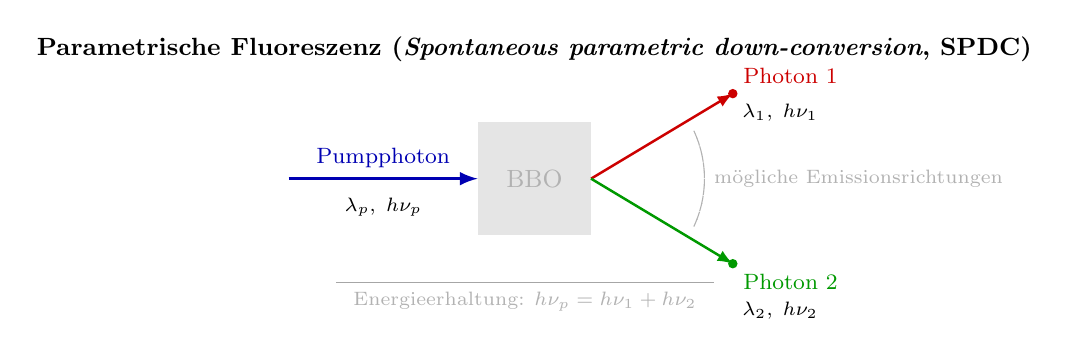
\begin{tikzpicture}[>=latex, scale=1.2]

% --- Farben ---
\definecolor{pumpcol}{rgb}{0,0,0.7}
\definecolor{signalcol}{rgb}{0.8,0,0}
\definecolor{idlercol}{rgb}{0,0.6,0}

% --- Kristall ---
\fill[gray!20] (0,0) rectangle (1.2,1.2);
\node[gray!60] at (0.6,0.6) {\small BBO};

% --- Pump photon (input) ---
\draw[->,line width=1.2pt,pumpcol] (-2,0.6) -- (0,0.6)
  node[midway,above,pumpcol]{\footnotesize Pumpphoton};
\node at (-1.0,0.3) {\scriptsize $\lambda_p, \; h\nu_p$};

% --- Downconverted photons (output) ---
\draw[->,line width=0.9pt,signalcol] (1.2,0.6) -- +(1.5,0.9)
  node[above right,signalcol]{\footnotesize Photon~1};
\draw[->,line width=0.9pt,idlercol] (1.2,0.6) -- +(1.5,-0.9)
  node[below right,idlercol]{\footnotesize Photon~2};

\node at (3.2,1.3) {\scriptsize $\lambda_1, \; h\nu_1$};
\node at (3.2,-0.8) {\scriptsize $\lambda_2, \; h\nu_2$};

% --- Energy conservation symbolically ---
\draw[-,gray!70] (-1.5,-0.5) -- node[below,gray!60]{\scriptsize Energieerhaltung: $h\nu_p = h\nu_1 + h\nu_2$} (2.5,-0.5);

% --- Emission cones hint ---
\draw[gray!60,dashed,domain=-25:25] plot ({1.2 + 1.2*cos(\x)}, {0.6 + 1.2*sin(\x)});
\draw[gray!60,dashed,domain=-25:25] plot ({1.2 + 1.2*cos(\x)}, {0.6 - 1.2*sin(\x)});
\node[gray!60,right] at (2.4,0.6) {\scriptsize m\"ogliche Emissionsrichtungen};

% --- Detectors (optional) ---
\fill[signalcol] (2.7,1.5) circle(0.05);
\fill[idlercol] (2.7,-0.3) circle(0.05);
% \node[right,align=left] at (2.8,1.5) {\scriptsize Detektor 1};
% \node[right,align=left] at (2.8,-0.3) {\scriptsize Detektor 2};

% --- Label overall process ---
\node[above,yshift=0.4cm] at (0.6,1.4) {\small \textbf{Parametrische Fluoreszenz (\emph{Spontaneous parametric down-conversion}, SPDC)}};

\end{tikzpicture}
\caption{Schematische Darstellung der Erzeugung von Photonenpaaren in einem nichtlinearen BBO-Kristall.
Das Pumpphoton (blau) erzeugt zwei Photonen geringerer Energie, die unter Erhaltung von Energie und Impuls in charakteristischen Winkeln austreten.
Bei bestimmten Winkeln k\"onnen die beiden Photonen verschr\"ankt sein.}
\label{f:SPDC}
\end{figure}

Weitere Systeme, die einzelne Photonen emittieren k\"onnen, sind Halbleiter-Quantenpunkte (\glqq k\"unstliche Atome\grqq) und Farbzentren in Diamant (NV-Zentren). Bei den NV-Zentren handelt es sich um Punktdefekte im Kristall (\emph{Nitrogen Vacancy}), die auch in der Quantensensorik Anwendung finden.

\section{Interferenz von Photonen}
In einem Interferometer oder beim Doppelspalt scheint es, als w\"urde ein Photon mit sich selbst interferieren, da auch bei Einzelphotonexperimenten ein Interferenzmuster entsteht, wenn man gen\"ugend viele Einzelereignisse detektiert. Da ein Photon immer als ganzes Energiequant detektiert wird, sich also nicht teilt, ist das erstmal eine \"uberraschende Feststellung. Es ist nun hilfreich, sich zur Erkl\"arung des entstehenden Interferenzmusters mit der formalen Beschreibung des Zustands des Photons zu befassen. Die Interferenz basiert auf der Superposition der m\"oglichen Wege, die man sich f\"ur ein klassisches Teilchen vorstellen kann (Pfade im Interferometer (z.B.\ im Mach-Zehnder-Interferometer, Abb.\ \ref{f:Mach-Zehnder}); linker oder rechter Spalt beim Doppelspalt). Genauer gesagt interferieren die Wahrscheinlichkeitsamplituden, die diesen Wegen bei der Beschreibung des Photons zugeordnet werden.
Zur Veranschaulichung des Prinzips betrachten wir an dieser Stelle nur den Fall einer einzelnen Aufspaltung in zwei Wege (z.B.\ an einem Strahlteiler), die durch die Zust\"ande $\ket{1}$ und $\ket{2}$ dargestellt werden. Ein Photon befindet sich dann im Zustand $$\ket{\psi}=\frac{1}{\sqrt{2}}\left(\ket{1}+\exp(i\varphi)\ket{2}\right)\;,$$ wobei $\varphi$ eine Phasenverschiebung zwischen den Wegen beschreibt. Die Wahrscheinlichkeit, das Photon an einem Detektor D zu messen, ist $$P(D)=|\braket{D}{\psi}|^2=\frac{1}{2}|\braket{D}{1}+\exp(i\varphi)\braket{D}{2}|^2\;.$$ Dieser Ausdruck enth\"alt Interferenzterme zwischen $\ket{1}$ und $\ket{2}$.
\begin{figure}[h]
\centering
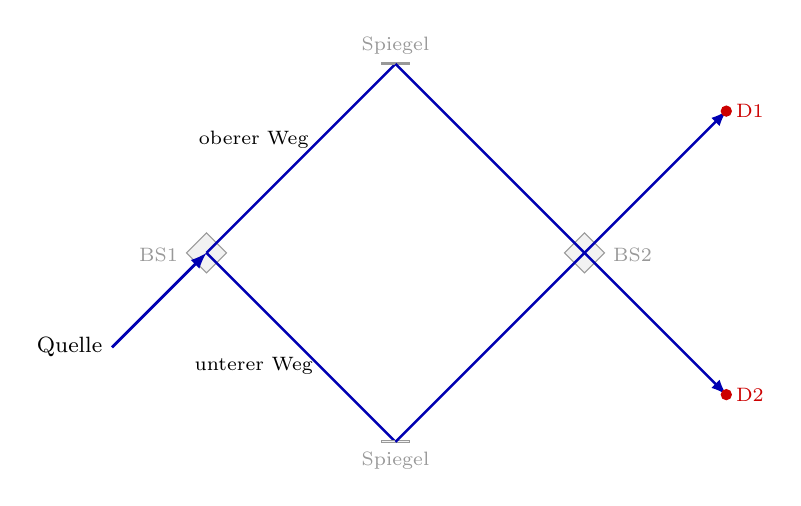
\begin{tikzpicture}[>=latex, scale=1.2]

% Farben
\definecolor{beam}{rgb}{0,0,0.7}
\definecolor{opt}{gray}{0.6}
\definecolor{det}{rgb}{0.8,0,0}

% Koordinaten
\coordinate (S)  at (-1,-1);
\coordinate (BS1) at (0,0);
\coordinate (M1)  at (2,2);
\coordinate (M2)  at (2,-2);
\coordinate (BS2) at (4,0);
\coordinate (D1)  at (5.5,1.5);
\coordinate (D2)  at (5.5,-1.5);

% BS1
\draw[opt, fill=gray!10, rotate=45] (-0.15,-0.15) rectangle (0.15,0.15);
% BS2
\draw[opt, fill=gray!10, shift={(4,0)}, rotate=45] (-0.15,-0.15) rectangle (0.15,0.15);
% Quelle
\node[left] at (S) {\footnotesize Quelle};
\draw[beam,->,line width=1pt] (S) -- (BS1);

\node[opt,above left] at (-0.2,-0.2) {\scriptsize BS1};

% Wege
\draw[beam,line width=0.9pt] (BS1) -- (M1);
\draw[beam,line width=0.9pt] (BS1) -- (M2);

% Spiegel
\draw[opt, fill=gray!10] (1.85,1.99) rectangle (2.15,2.01);
\node[opt,above] at (2,2) {\scriptsize Spiegel};

\draw[opt, fill=gray!10] (1.85,-1.99) rectangle (2.15,-2.01);
\node[opt,below] at (2,-2) {\scriptsize Spiegel};

% Rückwege
\draw[beam,line width=0.9pt] (M1) -- (BS2);
\draw[beam,line width=0.9pt] (M2) -- (BS2);

\node[opt,above right] at (4.2,-0.2) {\scriptsize BS2};

% Ausgänge
\draw[beam,->,line width=0.9pt] (BS2) -- (D1);
\draw[beam,->,line width=0.9pt] (BS2) -- (D2);

% Detektoren
\fill[det] (D1) circle (0.06);
\fill[det] (D2) circle (0.06);
\node[right,det] at (D1) {\scriptsize D1};
\node[right,det] at (D2) {\scriptsize D2};

% Wegbeschriftung
\node at (0.5,1.2) {\scriptsize oberer Weg};
\node at (0.5,-1.2) {\scriptsize unterer Weg};

% % Titel
% \node[above] at (2,1.9) {\small Mach--Zehnder--Interferometer};

\end{tikzpicture}
\caption{Schematisches Mach--Zehnder--Interferometer.
Nach dem ersten Strahlteiler (BS1) befindet sich das Photon in einer kohärenten Superposition zweier Wege.
Am zweiten Strahlteiler überlagern sich die zugehörigen Wahrscheinlichkeitsamplituden;
die Zählraten an den Detektoren D1 und D2 hängen von der relativen Phase der beiden Wege ab.}
\label{f:Mach-Zehnder}
\end{figure}

Das Interferenzmuster verschwindet allerdings, wenn es m\"oglich ist, festzustellen, welchen \glqq klassischen\grqq\ Weg das Photon genommen hat, wenn man also den Weg im Interferometer nachvollziehen oder den durchflogenen Spalt bestimmen kann. In der Zustandsbeschreibung erscheint die Markierung des Weges als Verschr\"ankung mit einem zus\"atzlichen Freiheitsgrad $$\ket{\Psi}=\frac{1}{\sqrt{2}}\left(\ket{1}\ket{M_1}+\exp(i\varphi)\ket{2}\ket{M_2}\right)\;.$$ Damit die Interferenz komplett verschwindet, m\"ussen $\ket{M_1}$ und $\ket{M_2}$ orthogonale Zust\"ande sein (sodass $\braket{M_1}{M_2}=0$; z.B.\ $\ket{H}$ und $\ket{V}$, wenn die Markierung \"uber die Polarisation der Photonen geschieht). Damit wird $$P(D)=\frac{1}{2}\left(|\braket{D}{1}|^2+|\braket{D}{2}|^2\right)\;,$$ was keine Interferenzterme mehr enth\"alt. Es ist dabei nicht n\"otig, den Weg tats\"achlich zu bestimmen, denn f\"ur das Verschwinden der Interferenz reicht allein die Existenz dieser M\"oglichkeit; man muss nicht wissen, ob der zus\"atzliche Freiheitsgrad $M_1$ oder $M_2$ war.

\paragraph{Hong-Ou-Mandel-Effekt}
Eine sich daraus ergebende Besonderheit stellt der Hong-Ou-Mandel-Effekt dar. Treffen zwei Photonen (exakt) gleichzeitig von zwei Seiten auf einen 50:50-Strahlteiler, verlassen sie diesen stets gemeinsam auf einer der beiden Seiten. Welche Seite das ist, ist dabei zuf\"allig, aber es ist ausgeschlossen, dass ein Photon auf der einen und eines auf der anderen Seite austritt. Der Grund hierf\"ur ist die destruktive \"Uberlagerung der Varianten \glqq beide Photonen werden reflektiert\grqq\ und \glqq beide Photonen werden transmittiert\grqq\footnote{Achtung: Es interferieren nicht die Photonen auf den Wegen, sondern die Amplituden der Zust\"ande \glqq beide reflektiert\grqq\ und \glqq beide transmittiert\grqq.}, Abb.\ \ref{f:HOM}. Man spricht auch von der unterdr\"uckten Koinzidenz. Ver\"andert man die Unterscheidbarkeit der Photonen oder die Auftreffzeitpunkte am Strahlteiler, kann es wieder Koinzidenzen geben. In Abh\"angigkeit des Zeitversatzes der Photonen findet man so eine Koinzidenzsenkung in der Umgebung von $\Delta t=0$.
\begin{figure}[h]
\centering
\begin{tikzpicture}[scale=1.0]

% Farben
\definecolor{opt}{gray}{0.60}
\definecolor{cancel}{rgb}{0.8,0,0}

% Titel
\node at (6,3.8) {\small \textbf{Hong--Ou--Mandel--Effekt: Interferenz von Zwei--Photonen--Amplituden}};

% ---------
% Hilfsfunktion: kleiner Strahlteiler
% ---------
\newcommand{\BS}[2]{
  % Strahlteiler
  \draw[opt, shift={(#1,#2)}, rotate=45] (-0.15,-0.15) rectangle (+0.15,+0.15);
}

% ---------
% Vier klassische Skizzen
% ---------

% (1) R,T
\BS{0}{2.5}
\draw (-0.5,3.0) -- (0,2.5);   % Photon A
\draw (-0.5,2.0) -- (0,2.5);   % Photon B
\draw (0,2.5) -- (0.5,3.0);
\draw (0,2.5) -- (0.5,3.0);
\node at (0,3.3) {\scriptsize (R,T)};

% (2) R,R
\BS{4}{2.5}
\draw (3.5,3.0) -- (4,2.5);
\draw (3.5,2.0) -- (4,2.5);
\draw (4,2.5) -- (4.5,3.0);
\draw (4,2.5) -- (4.5,2.0);
\node at (4,3.3) {\scriptsize (R,R)};

% (3) T,T
\BS{8}{2.5}
\draw (7.5,3.0) -- (8,2.5);
\draw (7.5,2.0) -- (8,2.5);
\draw (8,2.5) -- (8.5,2.0);
\draw (8,2.5) -- (8.5,3.0);
\node at (8,3.3) {\scriptsize (T,T)};

% (4) T,R
\BS{12}{2.5}
\draw (11.5,3.0) -- (12,2.5);
\draw (11.5,2.0) -- (12,2.5);
\draw (12,2.5) -- (12.5,2.0);
\draw (12,2.5) -- (12.5,2.0);
\node at (12,3.3) {\scriptsize (T,R)};

% Pluszeichen
\node at (2,2.5) {\Large $+$};
\node at (6,2.5) {\Large $+$};
\node at (10,2.5) {\Large $+$};

% ---------
% Amplituden
% ---------
\node at (0,1.2) {\scriptsize $+\tfrac{i}{\sqrt2}\,|2,0\rangle$};
\node at (4,1.2) {\scriptsize $+\tfrac{1}{\sqrt2}\,|1,1\rangle$};
\node at (8,1.2) {\scriptsize $-\tfrac{1}{\sqrt2}\,|1,1\rangle$};
\node at (12,1.2) {\scriptsize $\tfrac{i}{\sqrt2}\,|0,2\rangle$};

% Auslöschung markieren
\draw[cancel,thick] (3.2,0.7) -- (8.8,1.7);
\draw[cancel,thick] (3.2,1.7) -- (8.8,0.7);
\node[cancel] at (6,0.6) {\scriptsize destruktive Interferenz};

% Ergebnis
\node at (6,0)
{\scriptsize Ergebnis:
$\displaystyle |\psi_{\text{out}}\rangle
= \tfrac{1}{\sqrt2}\bigl(|2,0\rangle + |0,2\rangle\bigr)$};

\end{tikzpicture}
\caption{Vier klassische Alternativen für zwei gleichzeitig (von links) eintreffende Photonen an einem symmetrischen 50:50-Strahlteiler.
Die beiden Alternativen, die klassisch zu je einem Photon pro Ausgang führen würden,
sind quantenmechanisch ununterscheidbar und tragen Amplituden mit entgegengesetztem Vorzeichen.
Sie interferieren destruktiv, sodass der Koinzidenzterm \(|1,1\rangle\) verschwindet. Die Bra-Ket-Notation $\ket{k,~l}$ bezeichnet den Fall, dass $k$ Photonen im oberen Detektor landen und $l$ Photonen im unteren. (R,T) bezeichnet die klassische M\"oglichkeit, dass Photon 1 reflektiert und Photon 2 transmittiert wird (etc.).}
\label{f:HOM}
\end{figure}

\section{Photoelektrischer Effekt}
Der photoelektrische Effekt bezeichnet das experimentell beobachtete Ausl\"osen von Elektronen aus einer Metalloberfl\"ache durch einfallendes Licht. Dieses Ph\"anomen lie{\ss} sich mit der klassischen Wellentheorie des Lichts nicht vereinbaren: Unterhalb einer materialspezifischen Grenzfrequenz tritt kein Elektronenaustritt auf, unabh\"angig von der Lichtintensit\"at, w\"ahrend oberhalb dieser Frequenz die maximale kinetische Energie der Elektronen linear mit der Frequenz des Lichts zunimmt.

Albert Einstein gab 1905 eine theoretische Deutung dieses Effekts, für die ihm 1921 der Nobelpreis f\"ur Physik verliehen wurde~\cite{nobel1921}. Er nutzte dazu die Beziehung \(E = h\nu\) und interpretierte die Energie\"ubertragung zwischen Licht und Materie als grunds\"atzlich diskret.

Der photoelektrische Effekt macht damit die Quantisierung der Energie\"ubertragung deutlich, im Gegensatz zur Interferenz, die die koh\"arente \"Uberlagerung von Zust\"anden hervorhebt. Allerdings l\"asst sich der Effekt auch in einer semiklassischen Beschreibung erkl\"aren, in der die Elektronen quantenmechanisch, das elektromagnetische Feld jedoch klassisch behandelt wird. Er allein erzwingt daher noch keine vollst\"andige Quantisierung des Lichtfeldes.

\section{Wie kann man sich ein Photon (nicht) vorstellen?}
Wir wissen, dass ein Photon eine Energie von $E_{\rm Ph}=\hbar\omega=h\nu$ hat, dass es einen Impuls von $p=E_{\rm Ph}/c$ hat (relativistisch zu betrachtendes Objekt), dass es einen Polarisationszustand haben kann und dass es Interferenz zeigen kann. Es w\"are aber falsch, sich vorzustellen, dass es sich um ein m\"oglicherweise kugelf\"ormiges Teilchen handelt oder auch, dass es ein kleiner Teil einer elektromagnetischen Welle ist. Es ist auch kein Teilchen, das auf einer Welle \glqq reitet\grqq. Es gibt keine wohldefinierte Ausdehnung oder \glqq Gr\"o{\ss}e\grqq\ des Photons - die r\"aumliche Lokalisierung entsteht h\"ochstens durch die Beschreibung als Wellenpaket (also seine Modenverteilung). Es gibt auch keine klassische Bahnkurve, entlang der sich ein Photon bewegt, sondern nur Wahrscheinlichkeitsaussagen \"uber das Detektieren eines Photons an einem Ort zu einer Zeit.

Eine pr\"azise mathematische Beschreibung des Photons erh\"alt man als einzelne Anregung eines quantisierten elektromagnetischen Feldmodus, also als Fock-Zustand des Feldes.
F\"ur einen einzelnen Modus lautet der Hamilton-Operator
\[
\hat{H}=\hbar\omega\left(\hat{a}^\dagger\hat{a}+\frac{1}{2}\right),
\]
wobei $\hat{a}^\dagger$ und $\hat{a}$ Erzeugungs- bzw.\ Vernichtungsoperatoren sind und
$\left[\hat{a},\hat{a}^\dagger\right]=1$ gilt. Diese Operatoren wirken auf die Eigenzust\"ande $\ket{n}$ wie folgt:
\begin{align}
\hat{a}^\dagger\ket{n}&=\sqrt{n+1}\ket{n+1}\\
\hat{a}\ket{n}&=\sqrt{n}\ket{n-1}\;,
\end{align}
$n$ z\"ahlt dabei die Photonen im selben Modus (definiert durch Frequenz und Polarisation). Der Photonenzahloperator $\hat{N}:=\hat{a}^\dagger\hat{a}$ liefert dann beispielsweise
\begin{align}
\hat{N}\ket{1} &= \hat{a}^\dagger\hat{a}\ket{1}\\
&= \hat{a}^\dagger 1\ket{0}\\
&= 1\ket{1}\;,
\end{align}
wobei $\ket{0}$ als Vakuumzustand bezeichnet wird; siehe Abb.\ \ref{f:Quant_Modus}.
\begin{figure}[h]
\centering
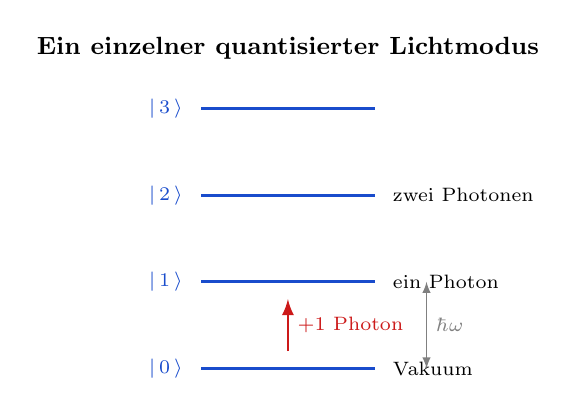
\begin{tikzpicture}[>=latex, scale=1.1]

% Farben
\definecolor{modeblue}{rgb}{0.1,0.3,0.8}
\definecolor{photonred}{rgb}{0.8,0.1,0.1}

% Titel
\node at (0,4.2) {\small \textbf{Ein einzelner quantisierter Lichtmodus}};

% Energieniveaus (Leiter)
\foreach \n/\y in {0/0.5,1/1.5,2/2.5,3/3.5} {
  \draw[modeblue, line width=1pt] (-1,\y) -- (1,\y);
  \node[left,modeblue] at (-1.1,\y) {\scriptsize $|\,\n\,\rangle$};
}

% Beschriftungen
\node[right] at (1.1,0.5) {\scriptsize Vakuum};
\node[right] at (1.1,1.5) {\scriptsize ein Photon};
\node[right] at (1.1,2.5) {\scriptsize zwei Photonen};

% Energieabstände
\draw[<->,gray] (1.6,0.5) -- (1.6,1.5);
\node[right,gray] at (1.6,1.0) {\scriptsize $\hbar\omega$};

% Photon hinzufügen
\draw[photonred,->,line width=1pt] (0,0.7) -- (0,1.3);
\node[photonred,right] at (0,1.0) {\scriptsize $+1$ Photon};

\end{tikzpicture}
\caption{Darstellung eines einzelnen quantisierten Lichtmodus.
Die Zustände \(\ket{n}\) unterscheiden sich durch die Anzahl der Anregungen dieses Modus.
Ein Photon entspricht dem Übergang vom Vakuumzustand \(\ket{0}\) zum Zustand \(\ket{1}\);
jede weitere Anregung erhöht die Energie um \(\hbar\omega\).}
\label{f:Quant_Modus}
\end{figure}

Um reine Einzelphotonenzust\"ande zu erzeugen, reicht es nicht aus, die Intensit\"at einer Lichtquelle immer weiter zu reduzieren. Dieses Vorgehen resultiert i.A.\ in einer Verteilung verschiedener Zust\"ande $\ket{0}$, $\ket{1}$, $\ket{2}$, $\ldots$. Bei einem Laser ergibt sich z.B.\ eine Poissonverteilung der Photonenzahlen. Au{\ss}erdem zeigen echte Einzelphotonen sogenanntes Anti-Bunching, schwaches koh\"arentes Licht jedoch nicht. Diese Eigenschaft bezieht sich auf den Wert der zeitlichen Intensit\"atskorrelationsfunktion $g^{(2)}(\tau)$ f\"ur $\tau\to 0$:
\begin{align}
g^{(2)}(0)=\dfrac{\langle \hat{N}(\hat{N}-1)\rangle}{\langle \hat{N}\rangle^2}
% \begin{cases}
% = 1,\quad\text{kein Anti-Bunching}\;,\\
% < 1,\quad\text{Anti-Bunching}\;.
% \end{cases}
\end{align}
F\"ur koh\"arentes Licht ist $g^{(2)}(0)=1$, f\"ur einen idealen Einzelphotonenzustand $g^{(2)}(0)=0$.
Ein Einzelphotonenzustand ist somit nicht einfach \glqq sehr schwaches Licht\grqq\,
sondern ein spezifischer Quantenzustand des elektromagnetischen Feldes.

Zusammenfassend ist ein Photon weder ein klassisches Teilchen noch ein abgeschnittenes St\"uck einer Welle.
Es ist eine diskrete Anregung eines bestimmten Feldmodus,
dessen r\"aumliche und zeitliche Struktur durch diesen Modus festgelegt ist.
Je nach experimenteller Anordnung treten Eigenschaften hervor,
die an Wellenph\"anomene (Interferenz, Superposition) oder an Teilchenph\"anomene
(diskrete Energie\"ubertragung, Anti-Bunching) erinnern.

\newpage
\section*{Literaturempfehlung}
\begin{itemize}
\item R. Loudon: The Quantum Theory of Light. Oxford University Press.
\item C.K. Hong, Z.Y. Ou, L. Mandel (1987), Measurement of Subpicosecond Time Intervals between Two Photons by Interference, Phys. Rev. Lett. 59, 2044.
\item M.O. Scully, M. Suhail Zubairy: Quantum Optics. Cambridge University Press.
\end{itemize}

\begin{thebibliography}{99}
\bibitem{nobel1921} The Nobel Prize in Physics 1921. NobelPrize.org. Nobel Prize Outreach 2026. Sun. 18 Jan 2026. \url{https://www.nobelprize.org/prizes/physics/1921/summary/}
\end{thebibliography}

\end{document}

